%!TEX root = ../root.tex

\section{This is a section}
\blindtext \myfootcite[Vgl.][42]{example}
\subsection{This is a subsection}
\blindtext \ac{API}
\subsubsection{This is a subsubsection}
\blindtext \acp{API}
\section*{This is a unnumbered section}

\begin{figure}[ht] 
    \centering
    \caption{Example caption}
    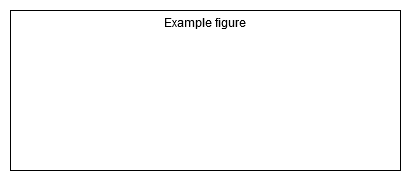
\includegraphics[width=\textwidth]{figure.png} 
    \subcaption{Source: \mycite[69]{example}}
    \label{fig:goodreference}
\end{figure}

\blindtext

\begin{subcaptionenv}{Source: \mycite[Vgl.][2]{example}}
    \begin{lstlisting}[caption={Express Example}, language=javascript]
const express = require('express')
const app = express()
const port = 3000

app.get('/', (req, res) => res.send('Hello World!'))

app.listen(port, () => console.log(`Example app listening on port ${port}!`))
    \end{lstlisting}
\end{subcaptionenv}

\blindtext

\begin{figure}[h]
    \centering
    \caption{Plantuml test}
    \begin{plantuml}
        @startuml

        box "Machine"
            participant "Sensors" as sensors
            participant "OPC UA Server" as opc
        end box
        participant "Cloud" as cloud

        sensors <-> opc
        opc <-> cloud

        @enduml    
    \end{plantuml}
    \caption*{\footnotesize{Quelle: \mycite[69]{example}}}
    \label{fig:plantuml_test}
\end{figure}

\ifdebug{}debug ist an\fi

\section{lol}
\section{lol}
\section{lol}
\section{lol}
\section{lol}
\section{lol}
\section{lol}
\section{lol}
\section{lol}
\section{lol}
\section{lol}
\section{lol}
\section{lol}
\section{lol}
\section{lol}
\section{lol}
\section{lol}
\section{lol}
\section{lol}
\section{lol}
\section{lol}
